% Start backup slides
\section*{Backup Slides}
\backupbegin
\begin{frame}{Spike-by-Spike Neural Network}

			\begin{figure}
				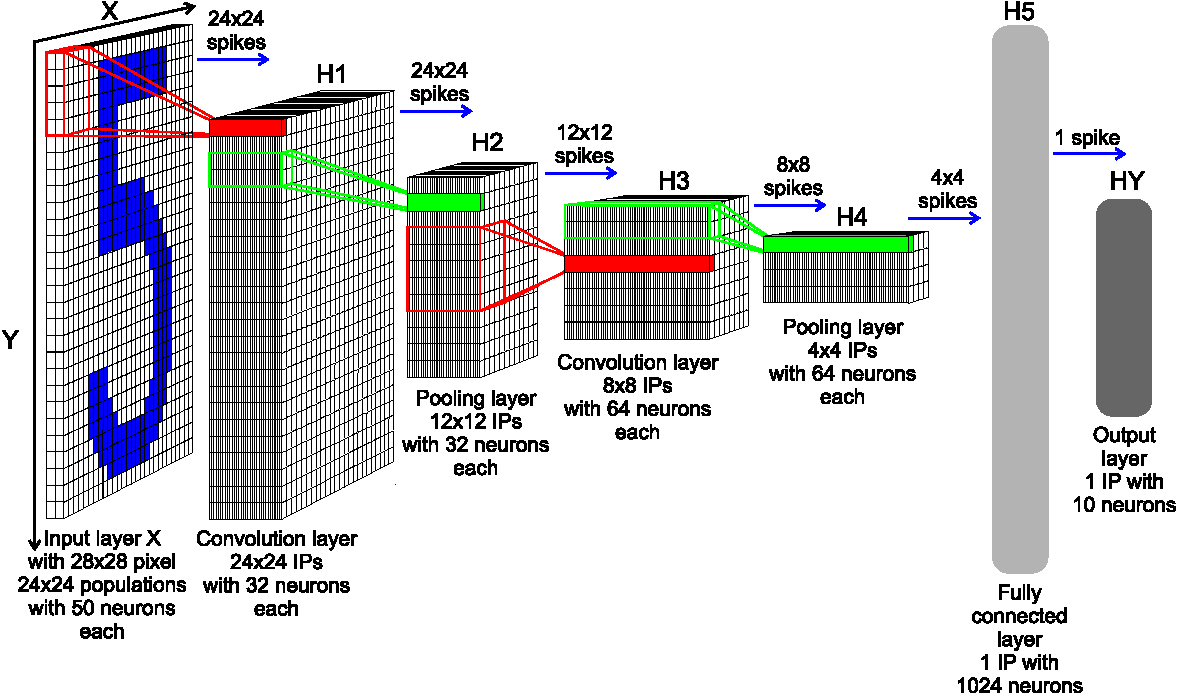
\includegraphics[width=0.9\textwidth]{../chapters/sbs_accelerator/figures/sbs_network.pdf} % Adjust the filename
				\caption{Spike-by-Spike (SbS) neural network architecture for handwritten digit classification task}
			\end{figure}

\end{frame}

\begin{frame}{SbS Processing Unit}
	\begin{columns}[c] % The [T] option aligns the tops of the columns
		
		% Left column for the first image
		\begin{column}<1->{0.5\textwidth}
			\begin{figure}
				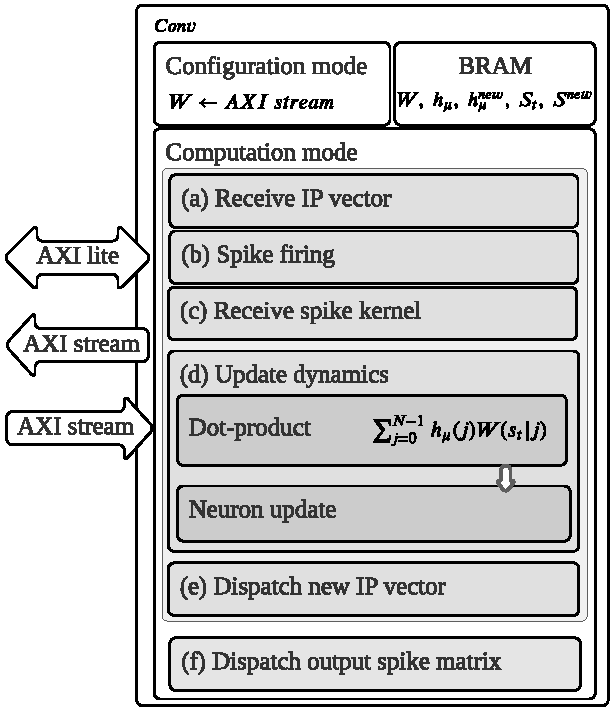
\includegraphics[width=0.7\textwidth]{../chapters/sbs_accelerator/figures/sbs_conv.pdf} % Adjust the filename
				\caption{Convolution processing unit}
			\end{figure}
		\end{column}
		
		% Right column for the second image
		\begin{column}<2->{0.5\textwidth}
			\begin{figure}
				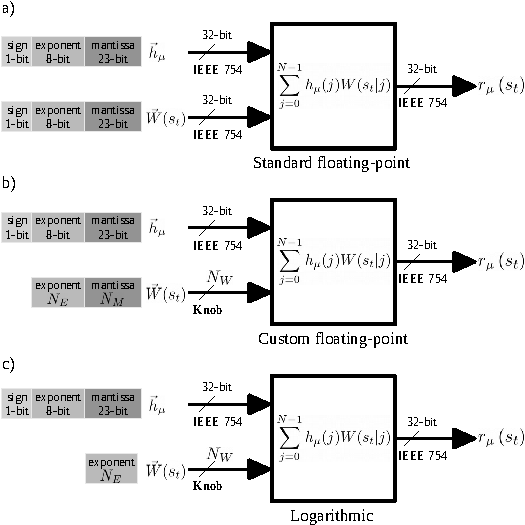
\includegraphics[width=0.9\textwidth]{../chapters/sbs_accelerator/figures/dot-product_unit.pdf} % Adjust the filename
				\caption{Dot-product hardware module}
			\end{figure}
		\end{column}
		
	\end{columns}
\end{frame}

\begin{frame}{Conv2D Tensor Processor}
	\begin{columns}[c] % The [T] option aligns the tops of the columns
		
		% Left column for the first image
		\begin{column}<1->{0.5\textwidth}
			\begin{figure}
				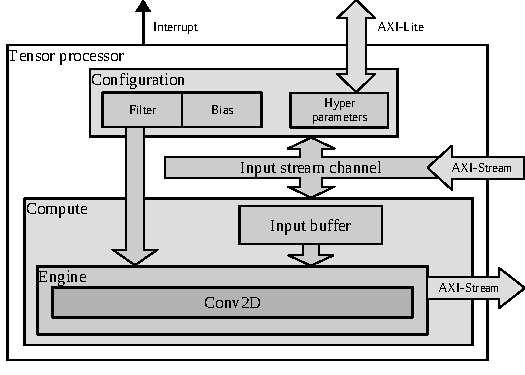
\includegraphics[width=0.7\textwidth]{../chapters/cnn_accelerator/figures/accelerator.pdf} % Adjust the filename
				\caption{High level architecture of tensor processor}
			\end{figure}
		\end{column}
		
		% Right column for the second image
		\begin{column}<2->{0.5\textwidth}
			\begin{figure}
				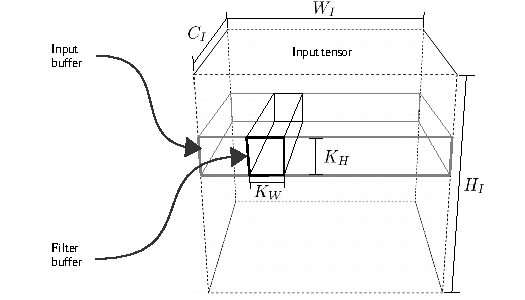
\includegraphics[width=0.9\textwidth]{../chapters/cnn_accelerator/figures/accelerator_buffers.pdf} % Adjust the filename
				\caption{ On-chip memory buffers}
			\end{figure}
		\end{column}
		
	\end{columns}
\end{frame}

\begin{frame}{Tensor Processor Setup Data Frame}
	
	\begin{figure}
		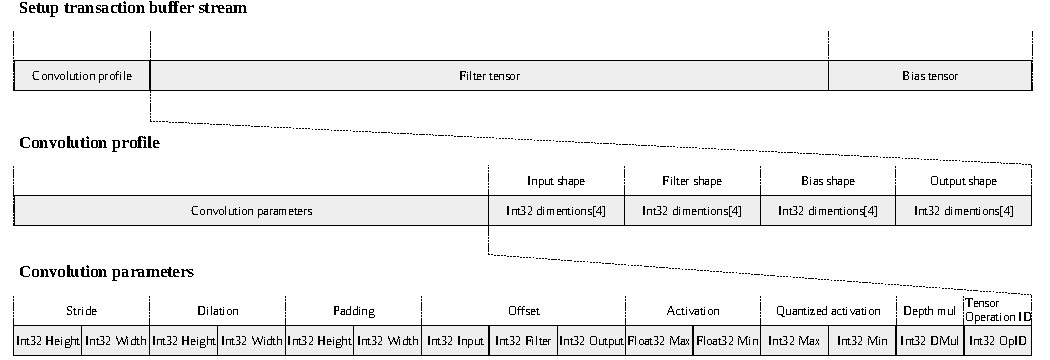
\includegraphics[width=\textwidth]{../figures/setup_transaction_buffer_stream.pdf}
		\caption{Setup transaction buffer stream}
	\end{figure}
	
\end{frame}


\begin{frame}{Embedded System Architecture with Tensor Processor}
	\begin{figure}
		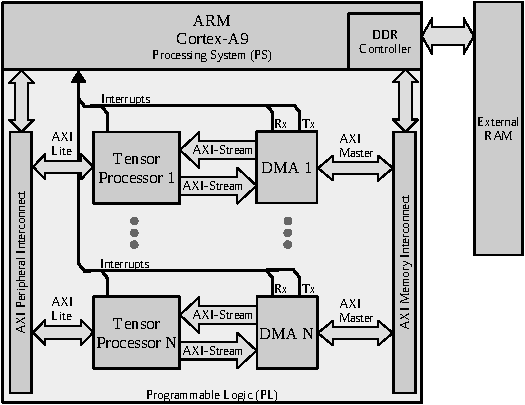
\includegraphics[width=0.75\textwidth]{../chapters/cnn_accelerator/figures/system_design.pdf} % Adjust the filename
		\caption{Embedded system architecture}
	\end{figure}
\end{frame}

\begin{frame}
	\frametitle{Comparison with Related Work with Tensor Processor} % optional, remove or leave empty if no title is desired
	\begin{center}
		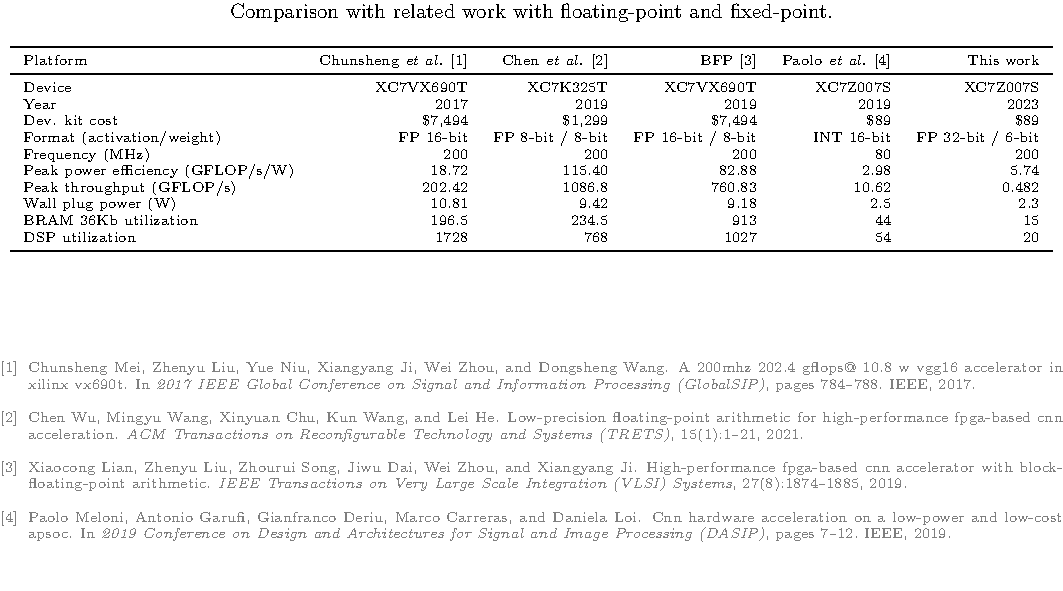
\includegraphics[width=\textwidth]{slides/figures/cnn_related_work.pdf} % Adjust the width as needed
	\end{center}
\end{frame}

\backupend